\section{Signal Start Detection}
\label{sec:03_signalStartDetection}

As mentioned in \ref{sec:02_signalStartDetection}, the detection of the
signal start is crucial for the localization.
The implementation of the different methods will be presented coupled with
an examination of real measurement data.
To reduce undesirable effects and demonstrate the simplest form, a sinusoidal
signal with $3000Hz$ is recorded by the microphones.

\subsubsection{Spectral Entropy}

The formula to calculate the spectral entropy of a signal is \ref{eq:02_entropy}.

\begin{figure}[ht]
	\centering
		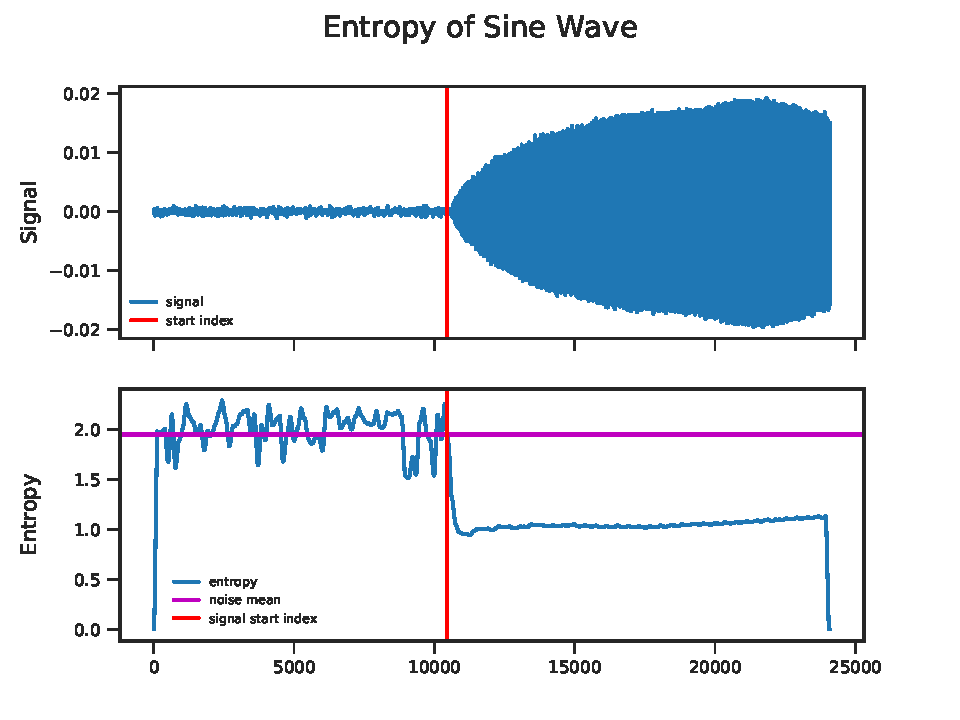
\includegraphics[width = 1.0 \columnwidth]{figures/example}
	\caption{Entropy of a sinusoidal signal with 3000Hz.}
\end{figure}
\label{fig:03_entropy}